\section{Análisis}

A la hora de experimentar, utilizamos nuestra implementación de traceroute sobre diversas universidades de todo el mundo, analizando distintas distancias y cantidades de saltos intercontinentales.

\subsection{China}

El primer análisis se hizo sobre la Universidad de Tsinghua en Pekín, República Popular de China. Su dirección web es \url{www.tsinghua.edu.cn}, la cual resolvía la dirección IP 166.111.4.100 a la hora de la experimentación. Debido a su lejanía, su análisis resulta interesante.

De los 28 saltos que se produjeron en el trazado, solamente 3 de ellos no generaron una respuesta, lo cual representa aproximadamente 10\% de los hosts. Los mismos se trataron de los primeros saltos, por lo que creemos que son hosts del ISP que no responden a este protocolo. Si ignoramos estos saltos nos queda una trayectoria con una longitud de 25 saltos.

\begin{figure}[H]
	\centering
	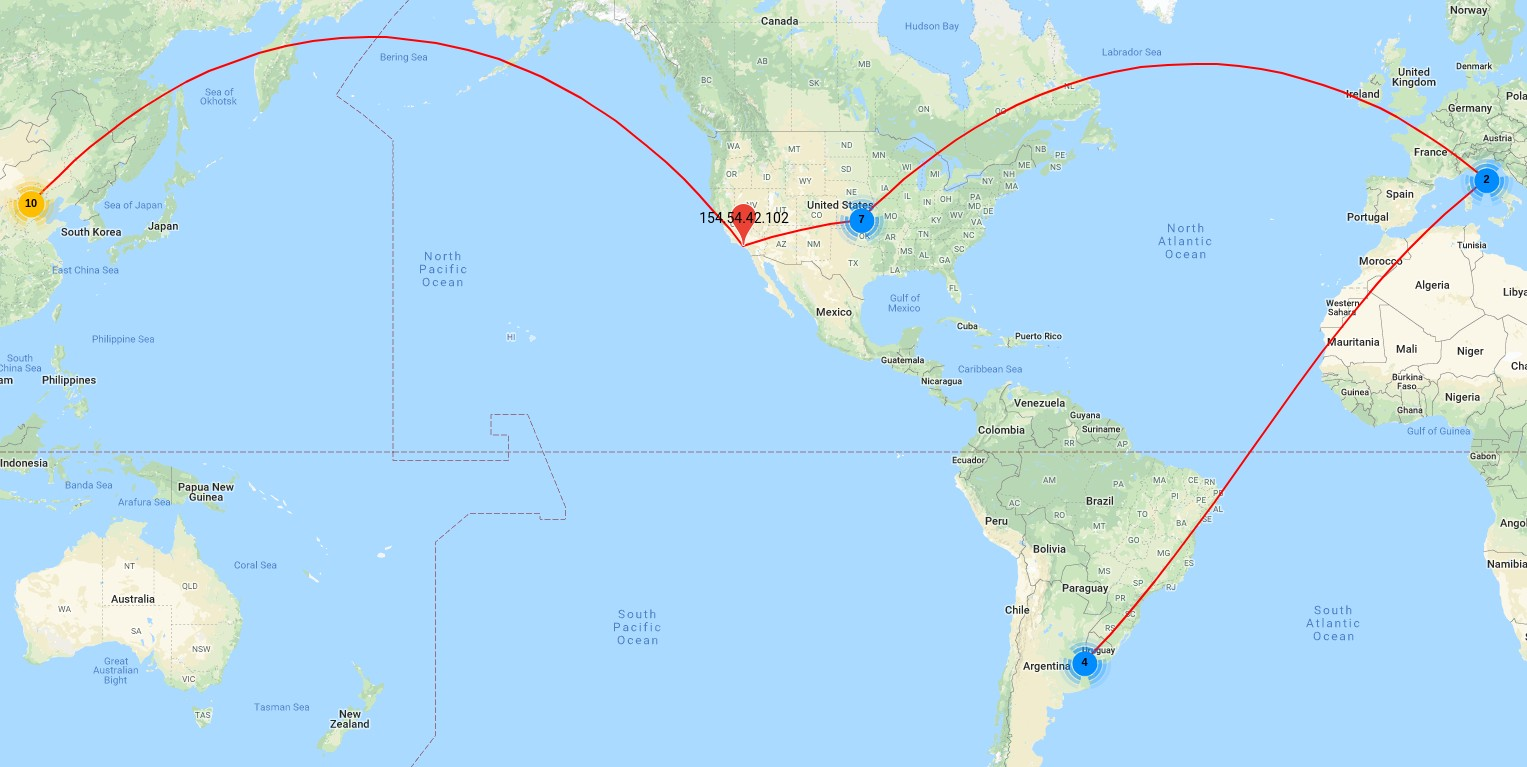
\includegraphics[width=.7\linewidth]{china_mapa.jpg}
	\captionsetup{justification=centering}
	\caption{Mapa de los nodos entre nuestros equipos y la Universidad de Tsinghua detectados por nuestro traceroute}
\end{figure}

En el mapa podemos ver un total de 3 saltos intercontinentales. Las direcciones IP fueron geolocalizadas usando los distintos servicios anteriormente nombrados. Resaltamos las direcciones IP 185.70.203.32 y 89.221.41.187, las cuales representan los host de los saltos 9 y 10 respectivamente. Para estas direcciones, hay servicios de geolocalización que dicen que ambas se encuentran en Italia, pero existen otros servicios que la ubican a la primera en Argentina y a la segunda en EE.UU. Estas direcciones IP pertenecen a la empresa Telecom Sparkle, originaria de Italia. Esta se encarga de mantener cables marinos, por lo que realmente no sabemos si realmente se encuentran en Italia o si algunos servicios la marcan como italiana solo por ser una empresa de dicho país.

Aplicando el método de Cimbala a la diferencia entre RTTs promedio de cada salto, detectamos como outliers los saltos con las correspondientes TTLs, 10 (89.221.41.187), 13 (154.54.84.1), 14 (154.54.30.162), 16 (154.54.44.86) y 19 (101.4.117.169). Lo primero que vimos es que el salto 9 no aparece como outlier, por lo que podríamos asumir que las direcciones IP tomadas como italianas tienen dicha localización por el origen de la empresa. Los saltos 13, 14 y 16 son saltos dentro de los Estados Unidos, por lo que podemos decir que el método introdujo falsos positivos. Finalmente el otro salto intercontinental desde norteamérica hacia asia fue el salto 19. Cuando aplicamos el método de forma no iterativa, solamente nos toma como outliers los puintos que realmente representan saltos intercontinentales, donde los RTTs incrementan de forma muy marcada.

\subsection{Inglaterra}

Este experimento corresponde a la Universidad de Oxford, Inglaterra. Más especificamente, nuestro traceroute es a la dirección \url{www.ox.ac.uk}.

De los 27 hops que observamos hubo 7 que no respondieron Time Exceeded, es casi el 26 \% de los host. 3 hosts pertenecen al cluster correspondiente a Argentina, otros 3 a Estados Unidos y el último a Inglaterra.

Aqui podemos observar el recorrido trazado en el planisferio.

Al geolocalizar los hosts con nuestros servicios, en el planisferio se observa una ruta con 2 enlaces intercontinentales. Además nos llamó la atención el hecho de que se realice un salto hacia Estados Unidos existiendo un cable submarino desde Brasil a Portugal. Pensamos que podria deberse a que es el único de Sudamérica hacia Europa y podría estar congestionado, mientras que desde Estados Unidos a Europa existen una cantidad considerable de enlaces submarinos.

\begin{figure}[H]
	\begin{minipage}{.5\textwidth}
		\centering
		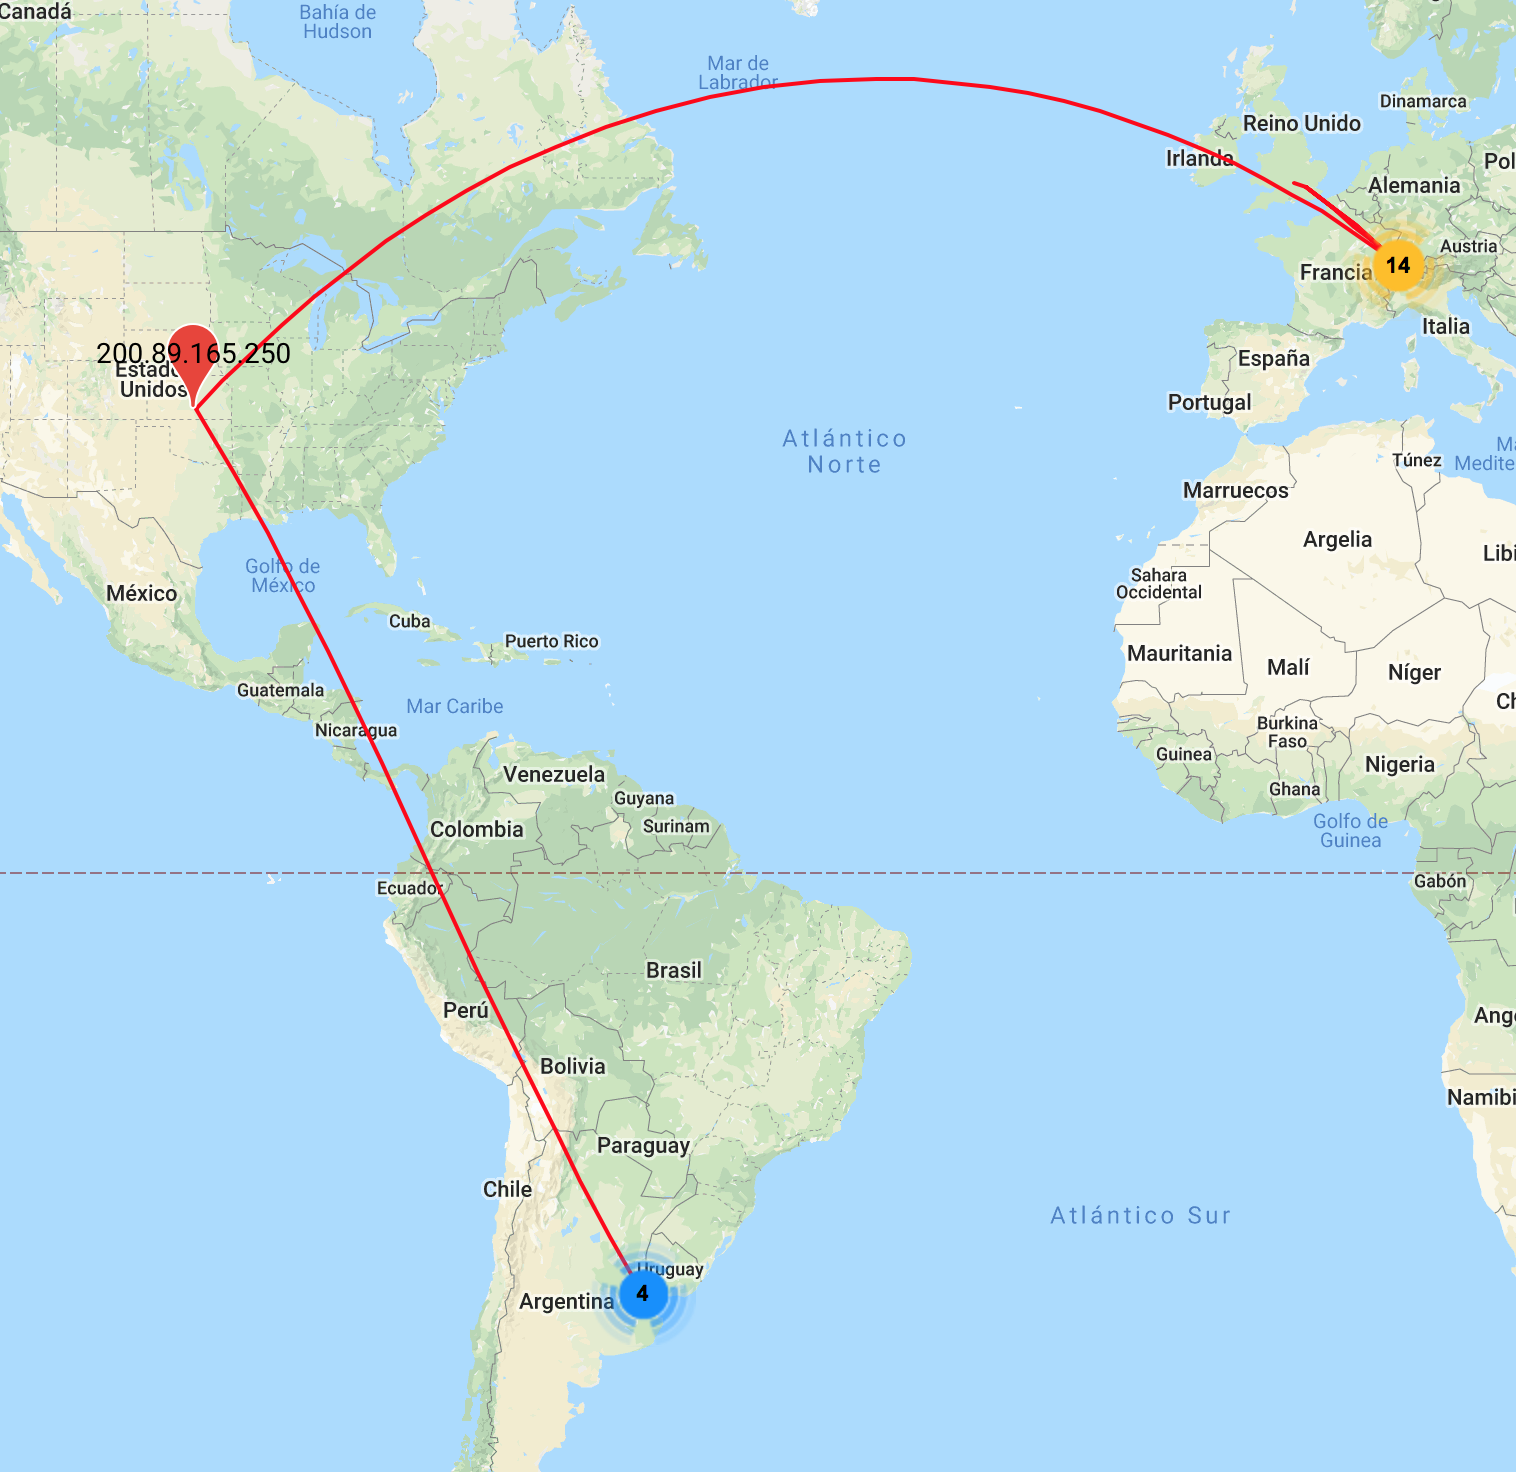
\includegraphics[width=.8\linewidth]{oxford_mapa.jpg}
	\end{minipage}%
	\begin{minipage}{.5\textwidth}
		\centering
		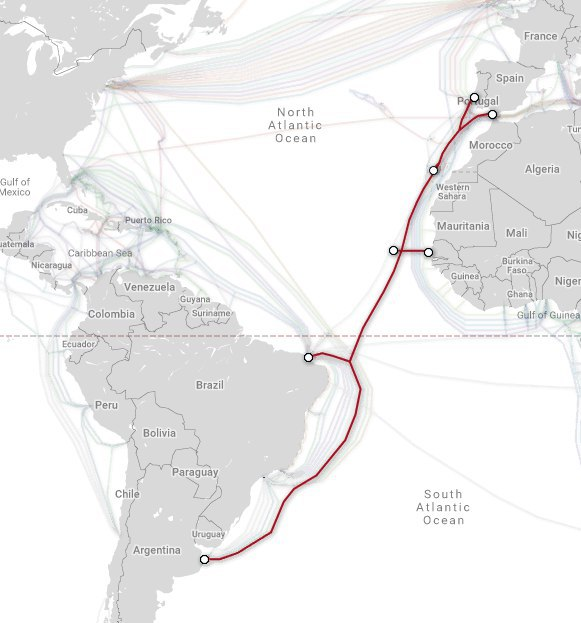
\includegraphics[width=.8\linewidth]{submarine_cable.jpg}
	\end{minipage}
	\captionsetup{justification=centering}
	\caption{Mapa de los nodos detectados entre nuestros equipos y la Universidad de Oxford (izquierda); y cable submarino disponible entre América del Sur y Europa (derecha; fuente: \url{https://submarinecablemap.com})}
\end{figure}


La distribución de RTT entre saltos presenta 3 outliers según el método Cimbala, lo cual no concuerda con la cantidad de saltos transoceánicos que se efectúan, que eran 2. El falso positivo es un salto que se produce dentro del cluster de argentina, la dirección 200.89.165.86. Sin embargo, al aplicar el método de forma no-iterativa, la cantidad de outliers se reduce a 1, es decir, tampoco representa correctamente los saltos intercontinentales. Es posible que esto se deba a la cantidad de nodos que no contestan, lo cual afecta el promedio y el tau de Thompson.

\subsection{EE.UU.}

El último experimento fue realizado con destino a analizar el trazado de rutas a la universidad de Stanford ubicada en los Estados Unidos, cuya web es stanford.edu. Este experimento, al tener una menor cantidad de saltos intercontinentales, es de sumo interés para ver cómo se comportan las tecnicas de deteccion en estos ambientes.

De los 18 saltos en la ruta solamente 5 no contestaron, y mantenemos los primeros 3 saltos sin contestar (posiblemente por el ISP), por lo que en este caso tenemos un 28\% de hosts que no contestan.

\begin{figure}[H]
	\centering
	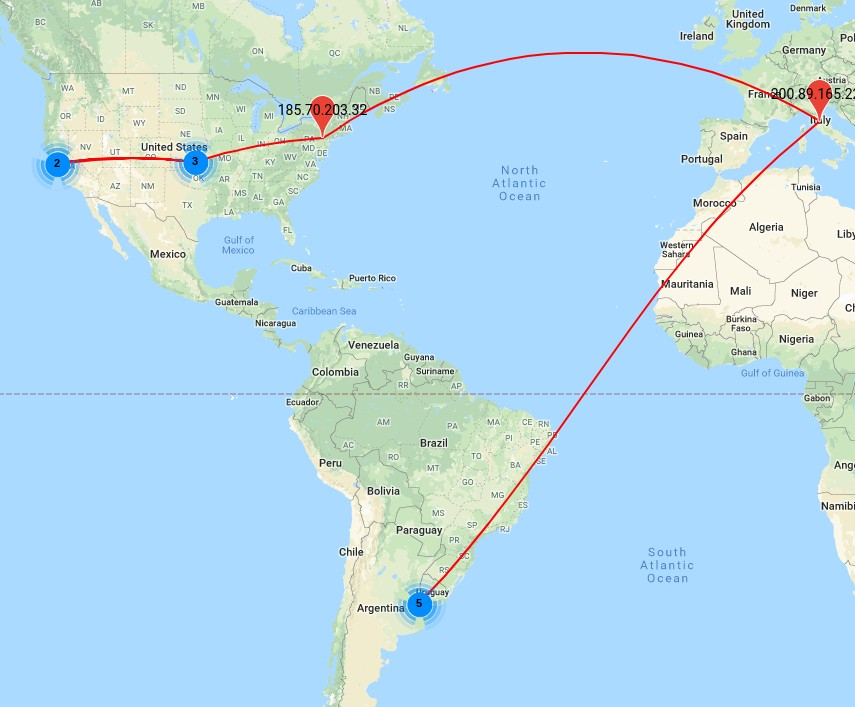
\includegraphics[width=.5\linewidth]{stanford_mapa.jpg}
	\captionsetup{justification=centering}
	\caption{Mapa de los nodos detectados entre nuestros equipos y la Universidad de Stanford}
\end{figure}

Una vez más, en el mapa se puede apreciar que uno de los hosts está teóricamente localizado en Italia. Dado que no es un salto lógico, y en base a nuestras observaciones anteriores, es seguro asumir que este dato es incorrecto, y en realidad se observa un único salto intercontinental (a América del Norte), y otro salto intermedio dentro de EE.UU. 

En el experimento podemos apreciar contrastando contra los ya nombrados servicios, que hay solamente un salto intercontinental. Cuando aplicamos el método de Cimbala para la detección de outliers, nos encontramos con 2 outliers, el del salto con TTL 5 (200.89.161.129) y TTL 10 (216.66.3.29), el segundo es realmente un salto intercontinental, conectando América del Norte con América del Sur, pero el segundo no es un salto intercontinental. Esto podría corresponder con el mencionado salto interno en EE.UU., ya que el tiempo de respuesta del host es alto. Sin embargo, al ser un salto por tierra, es probable que el salto no esté siendo correctamente representado, ya que los saltos anteriores no contestaron y la demora la de dichos hosts se acumula es un único hop. Al usar la versión no iterativa del método, este salto desaparece al ser de mucho menor impacto que el salto intercontinental.